% !TeX root = main.tex
\section{使用命令行编译}

\subsection{调出命令行工具}

\begin{frame}\frametitle{打开终端}
  \begin{description}
    \item[Windows 用户] 
    \begin{itemize}
      \item \keys{\win + S} 后输入 ``cmd'' 并按下回车, 可以打开``命令提示符'', 也就是所谓的命令行, 或者使用 \keys{\ctrl + \shift + \enter} 来用管理员权限打开命令行.
      \item 在``文件资源管理器''的地址栏输入``cmd'' 并按下回车, 即可在当前位置打开命令行:
      \item 如果安装了 Windows Terminal, 或者系统为 Win11, 可以在文件夹中或者文件夹上点击右键, 选择``在终端中打开'', 即可打开 Windows Terminal:
    \end{itemize}
    \item[macOS 用户] \keys{\cmdmac + \SPACE} 后输入``terminal'', 即可打开终端. 
    \item[Linux 用户] \keys{\ctrl + \Alt + T} 即可打开终端. 
  \end{description}
后面我们提到终端, 命令行均指这些东西, 并不做名字上的区分
\end{frame}


\begin{frame}[fragile]
  \frametitle{命令行操作}
  \begin{enumerate}
    \item \cmd{cd};
    \item \cmd{dir} (Windows), \cmd{ls} (Linux, macOS);
    \item \cmd{code}
  \end{enumerate}
\end{frame}


\begin{frame}[fragile]{使用命令行编译 \LaTeX 文件}
  \framesubtitle{第一次编译}
  \begin{enumerate}
    \item 在 \directory{D:/folder} 文件夹下新建 \directory{main.tex}, 输入以下内容
      \begin{latexcode}
      \documentclass{article}
      \begin{document}
        Hello \LaTeX!
      \end{document}  
      \end{latexcode}
    \item 在命令行中运行 
\begin{cmdcode}
pdflatex main.tex
\end{cmdcode}
      \begin{outputcode}
      This is pdfTeX, Version 3.141592653-2.6-1.40.24 (TeX Live 2022) (preloaded format=pdflatex)
      restricted \write18 enabled.
      entering extended mode
      (./main.tex
      LaTeX2e <2021-11-15> patch level 1
      L3 programming layer <2022-02-24>
      (/home/syvshclily/texlive/2022/texmf-dist/tex/latex/base/article.cls
      Document Class: article 2021/10/04 v1.4n Standard LaTeX document class
      (/home/syvshclily/texlive/2022/texmf-dist/tex/latex/base/size10.clo))
      (/home/syvshclily/texlive/2022/texmf-dist/tex/latex/l3backend/l3backend-pdftex.
      def) (./main.aux) [1{/home/syvshclily/texlive/2022/texmf-var/fonts/map/pdftex/u
      pdmap/pdftex.map}] (./main.aux) )</home/syvshclily/texlive/2022/texmf-dist/font
      s/type1/public/amsfonts/cm/cmr10.pfb>
      Output written on main.pdf (1 page, 12962 bytes).
      Transcript written on main.log. 
      \end{outputcode}
  \end{enumerate} 
\end{frame}

\subsubsection{遇到错误}

\begin{frame}[fragile]{使用命令行编译 \LaTeX 文件}
\framesubtitle{遇到错误}
  \begin{outputcode}
  This is pdfTeX, Version 3.141592653-2.6-1.40.24 (TeX Live 2022) (preloaded format=pdflatex)
  restricted \write18 enabled.
  entering extended mode
  (./main.tex
  LaTeX2e <2021-11-15> patch level 1
  L3 programming layer <2022-02-24>
  (/home/syvshclily/texlive/2022/texmf-dist/tex/latex/base/article.cls
  Document Class: article 2021/10/04 v1.4n Standard LaTeX document class
  (/home/syvshclily/texlive/2022/texmf-dist/tex/latex/base/size10.clo))
  (/home/syvshclily/texlive/2022/texmf-dist/tex/latex/l3backend/l3backend-pdftex.
  def) (./main.aux)
  ! Undefined control sequence.
  l.3   Hello \Latex
                    !
  ?  
  \end{outputcode}

  \begin{itemize}
    \item \keys{I + <cs> + \enter};
    \item \keys{X + \enter};
    \item \keys{H + \enter}.
  \end{itemize}
\end{frame}

\subsubsection{编译选项}

\begin{frame}[fragile]
  \frametitle{使用命令行编译 \LaTeX 文件}
  \framesubtitle{编译选项}

\begin{cmdcode}
pdflatex --option1 --option2=<string> main.tex
\end{cmdcode}
  
\begin{enumerate}
  \item \cmd{--synctex=1}
  \item \cmd{--jobname=<string>}
  \item \cmd{--output-directory=<string>}
  \item \cmd{--shell-escape}
  \item \cmd{--halt-on-error}
  \item \cmd{--interactionmode=<errorstop|scroll|batch|nonstop>mode}
\end{enumerate}
\end{frame}

\subsubsection{多次编译}

\subsubsection{多次编译}

\begin{frame}[fragile,t]
  \frametitle{使用命令行编译 \LaTeX 文件}
  \framesubtitle{目录与交叉引用}
\begin{latexcode}
% main.tex
\documentclass{article}
\begin{document}
\tableofcontents
\section{One}\label{sec:one}
  We are in section \ref{sec:one}
\end{document}
\end{latexcode}

\begin{onlyenv}<2>
\begin{cmdcode}
pdflatex main.tex
pdflatex main.tex
\end{cmdcode}  
\end{onlyenv}

\only<3>{
  \begin{center}
    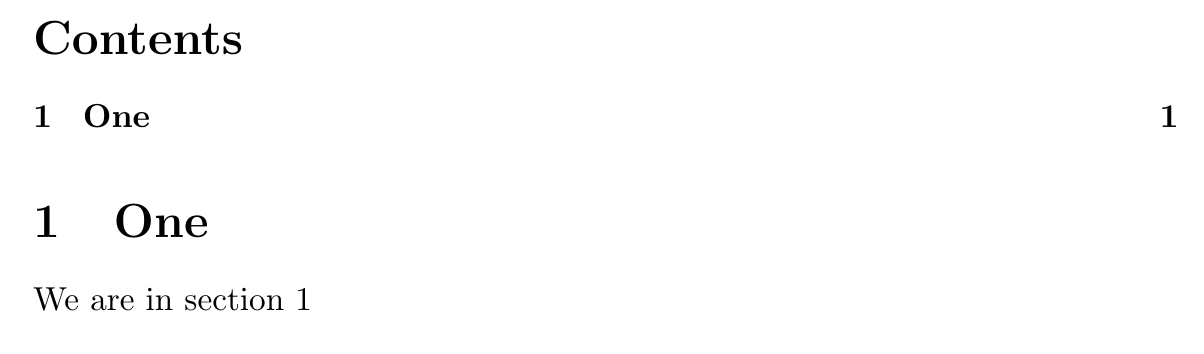
\includegraphics[height=3cm]{cross-ref-right.png}
  \end{center}
}
\end{frame}


\begin{frame}[fragile, t]
  \frametitle{使用命令行编译 \LaTeX 文件}
  \framesubtitle<1-3>{参考文献 --- \texttt{bibtex}}

\begin{onlyenv}<1-3>
\begin{latexcode}
\documentclass{article}
\begin{document}
  text\cite{article-full}
  \bibliographystyle{plain}
  \bibliography{xampl.bib}
\end{document}
\end{latexcode}
\end{onlyenv}

\begin{onlyenv}<2>
\begin{cmdcode}
pdflatex main.tex
bibtex main.aux
pdflatex main.tex
pdflatex main.tex
\end{cmdcode}  
\end{onlyenv}

\begin{onlyenv}<3>
  \begin{center}
    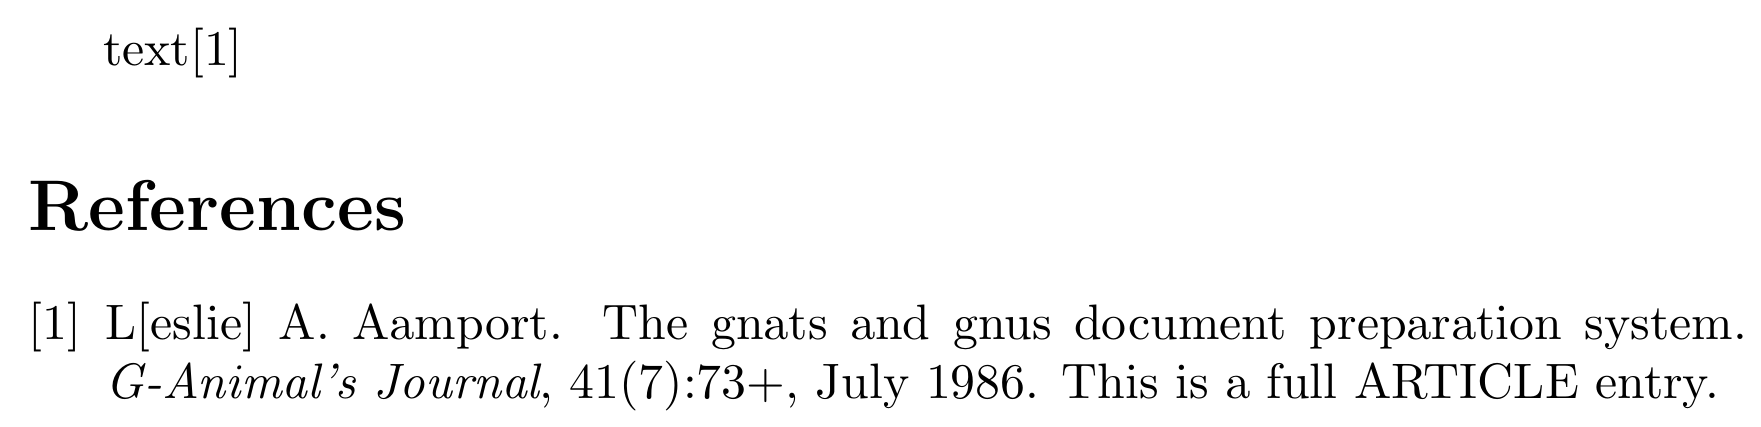
\includegraphics[width=\textwidth]{bibtex-ref.png}
  \end{center}
\end{onlyenv}

\framesubtitle<4-6>{参考文献 --- \texttt{biber}}

\begin{onlyenv}<4-6>
\begin{latexcode}
\documentclass{article}
\usepackage{biblatex}
\addbibresource{xampl.bib}
\begin{document}
  text\cite{article-full}
  \printbibliography
\end{document}
\end{latexcode}
\end{onlyenv}

\begin{onlyenv}<5>
  \begin{cmdcode}
  pdflatex main.tex
  biber main.bcf
  pdflatex main.tex
  pdflatex main.tex
  \end{cmdcode}  
  \end{onlyenv}
  
  \begin{onlyenv}<6>
    \begin{center}
      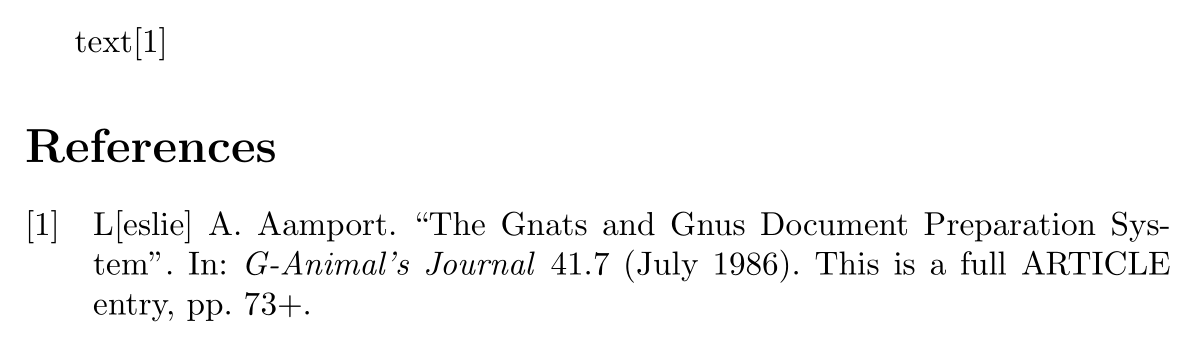
\includegraphics[width=\textwidth]{biber-ref.png}
    \end{center}
  \end{onlyenv}

\end{frame}

\subsubsection{更强大的工具: \texttt{latexmk}}

\begin{frame}[fragile]
  \frametitle{使用命令行编译 \LaTeX 文件}
  \framesubtitle{更强大的工具: \texttt{latexmk}}

\begin{onlyenv}<1>
\begin{latexcode}
% main.tex
\documentclass{article}
\begin{document}
\tableofcontents
\section{One}\label{sec:one}
  We are in section \ref{sec:one}, 
  and we have a cite \cite{article-full}
  \bibliographystyle{plain}
  \bibliography{xampl.bib}
\end{document}
\end{latexcode}

\begin{cmdcode}
latexmk -pdf main.tex
\end{cmdcode}
\end{onlyenv}

\begin{onlyenv}<2>  
\begin{latexcode}
% main.tex
\documentclass{ctexart}
\usepackage[style=gb7714-2015]{biblatex}
\addbibresource{xampl.bib}
\begin{document}
\tableofcontents
\section{测试节}\label{sec:one}
  我们现在是第 \ref{sec:one} 节,
  我们有一个引用 \cite{article-full}
  \printbibliography
\end{document}
\end{latexcode}

\begin{cmdcode}
latexmk -xelatex main.tex
\end{cmdcode}
\end{onlyenv}

\end{frame}

\subsubsection{更多}

\begin{frame}{使用命令行编译 \LaTeX 文件}
  \framesubtitle{更多的内容}
  latexmk 命令文件
  \begin{itemize}
    \item \cmd{latexmk -c}, \cmd{latexmk -C};
    \item \texttt{latexmkrc} 文件.
  \end{itemize}
  
  更多内容可以参见
  \begin{itemize}
    \item \texttt{\textbf{texdoc} latexmk}
    \item \cmd{pdflatex --help}
    \item \href{https://syvshc.github.io/2022-03-06-latex-terminal-compiling/}{在终端中编译 \LaTeX}
  \end{itemize}
\end{frame}

\section{使用 \tlmgr 进行包管理}

\begin{frame}[fragile]{\tlmgr 命令介绍}
\begin{itemize}
  \item \tlmgr 是 \texlive 用来管理\emph{软件包}的工具;
  \item \emph{软件包}指的不只是可以通过 \lcmd{\usepackage} 调用的宏包, 而是所有 \texlive 包含的, 可以使用 \tlmgr 管理的内容, 比如平常所说的宏包, 如 \lstinline{amsmath.sty}, 一些说明文档, 如 \lstinline{lshort-zh-cn}, 一些可执行文件, 如 \lstinline{xetex.exe} 等等.
  \item \tlmgr 是 \textbf{T}eX\textbf{L}ive \textbf{M}ana\textbf{g}e\textbf{r} 的缩写;
  \item 命令行中运行 \cmd{tlmgr version} 就可以看到当前的\emph{修订版号}(revision), 通常输出如下
\begin{outputcode}
tlmgr revision 63033 (2022-04-15 07:19:42 +0200)
tlmgr using installation: C:/texlive/2022
TeX Live (https://tug.org/texlive) version 2022
\end{outputcode}
\end{itemize}
\end{frame}

\subsection{\texttt{tlmgr} 的基本语法}

\begin{frame}[fragile]{\tlmgr 的基本语法}
\begin{cmdcode}
tlmgr -global-options action -action-specific-options operand
\end{cmdcode}
\begin{enumerate}
  \item \cmd{-} 与 \cmd{--} 相同;
  \item 顺序不重要;
  \item \cmd{-dry-run}.
\end{enumerate}
\end{frame}

\subsection{查看宏包信息}

\begin{frame}[fragile]{查看宏包说明信息 --- 操作: \frameaction{info}}
\begin{cmdcode}
tlmgr info pkg1 pkg2
\end{cmdcode}
  \begin{outputcode}
package:     elegantbook
category:    Package
shortdesc:   An Elegant LaTeX Template for Books
longdesc:    ElegantBook is designed for writing Books. This template is based on the standard LaTeX book class. The goal of this template is to make the writing process more elegant. Just enjoy it!
installed:   Yes
revision:    62989
sizes:       doc: 2613k, run: 49k
relocatable: No
cat-version: 4.3
cat-license: lppl1.3c
cat-topics:  class chinese book-pub
cat-contact-home: https://elegantlatex.org/
cat-contact-announce: https://elegantlatex.org/
cat-contact-repository: https://github.com/ElegantLaTeX/ElegantBook
cat-contact-support: https://github.com/ElegantLaTeX/ElegantBook/issues
collection:  collection-latexextra
  \end{outputcode}
  \end{frame}

\begin{frame}[fragile]{查看宏包说明信息 --- 操作: \frameaction{info}}

\begin{cmdcode}
tlmgr info -list pkg1 pkg2
\end{cmdcode}
\begin{outputcode}
# 省略 tlmgr info elegantbook 的内容 #
Included files, by type:
run files:
  texmf-dist/tex/latex/elegantbook/elegantbook.cls
doc files:
  texmf-dist/doc/latex/elegantbook/License
  texmf-dist/doc/latex/elegantbook/README-CN.md
  texmf-dist/doc/latex/elegantbook/README.md details="Readme"
  texmf-dist/doc/latex/elegantbook/elegantbook-cn.pdf details="Package documentation (Chinese)" language="zh"
  texmf-dist/doc/latex/elegantbook/elegantbook-cn.tex
  texmf-dist/doc/latex/elegantbook/elegantbook-en.pdf details="Package documentation (English)"
  texmf-dist/doc/latex/elegantbook/elegantbook-en.tex
  texmf-dist/doc/latex/elegantbook/figure/cover.jpg
  texmf-dist/doc/latex/elegantbook/figure/logo-blue.png
  texmf-dist/doc/latex/elegantbook/image/founder.png
  texmf-dist/doc/latex/elegantbook/image/scatter.jpg
  texmf-dist/doc/latex/elegantbook/reference.bib
\end{outputcode}
\end{frame}


\begin{frame}[fragile]{修改宏包更新源 --- 操作: \frameaction{option}}

\begin{cmdcode}
tlmgr option repository mirror
\end{cmdcode}

值得一提: \cmd{repository} = \cmd{repo}
\end{frame}

\begin{frame}[fragile]{更新软件包 --- 操作: \frameaction{update}}
\framesubtitle{查看哪些软件包可以更新}

\begin{cmdcode}
tlmgr update -list
\end{cmdcode}
\begin{outputcode}
tlmgr.pl: package repository https://mirrors.tuna.tsinghua.edu.cn/CTAN/systems/texlive/tlnet (not verified: gpg unavailable)
tlmgr.pl: would save backups to C:/texlive/2022/tlpkg/backups
tlmgr.pl: skipping forcibly removed package: collection-texworks
update:   adjmulticol   [316k]: local:  62935, source:  63073
update:   hitex         [2565k]: local:  62529, source:  63073
update:   texlive-fr    [1394k]: local:  62853, source:  63071
update:   texlive-msg-translations [144k]: local:  63010, source:  63072
update:   texlive-scripts.win32 [36k]: local:  62199, source:  63068
update:   texlive-scripts [504k]: local:  63049, source:  63068
update:   utfsym         [4766k]: local:  56729, source:  63076
update:   xduts          [871k]: local:  63013, source:  63075
update:   zwpagelayout   [641k]: local:  53965, source:  63074  
\end{outputcode}
\end{frame}

\begin{frame}[fragile]{更新软件包 --- 操作: \frameaction{update}}
\framesubtitle{更新全部软件包}

\begin{cmdcode}
tlmgr update -self -all
\end{cmdcode}
\begin{outputcode}
tlmgr.pl: package repository https://mirrors.tuna.tsinghua.edu.cn/CTAN/systems/texlive/tlnet (not verified: gpg unavailable)
tlmgr.pl: saving backups to C:/texlive/2022/tlpkg/backups
tlmgr.pl: no self-updates for tlmgr available
[ 1/16, ??:??/??:??] update: babel-french [567k] (59997 -> 63088) ... done
[ 2/16, 00:02/01:48] update: l3backend [894k] (63025 -> 63089) ... done
...
[16/16, 01:23/01:23] update: collection-luatex [1k] (62829 -> 63081) ... done
running mktexlsr ...
done running mktexlsr.
running mtxrun --generate ...
done running mtxrun --generate.
running updmap-sys ...
...
tlmgr.pl: package log updated: C:/texlive/2022/texmf-var/web2c/tlmgr.log
tlmgr.pl: command log updated: C:/texlive/2022/texmf-var/web2c/tlmgr-commands.log
\end{outputcode}
\end{frame}

\begin{frame}[fragile]{更新软件包 --- 操作: \frameaction{update}}
\framesubtitle{其他的功能}
\begin{enumerate}
\item 更新软件包 \pkg{pkg1}, \pkg{pkg2}:
\begin{cmdcode}
tlmgr update pkg1 pkg2
\end{cmdcode}
\item 如果更新全部宏包时不想更新 \pkg{pkg1}, \pkg{pkg2}:
\begin{cmdcode}
tlmgr update -self -all -exclude pkg1 -exclude pkg2
\end{cmdcode}
\item 如果更新过程被中断
\begin{cmdcode}
tlmgr update -self -all -reinstall-forcibly-removed
\end{cmdcode}
\end{enumerate}
\end{frame}


\subsection{回滚软件包的版本}

\begin{frame}[fragile]
  \frametitle{回滚软件包的版本 --- 操作: \frameaction{restore}}
  
  \framesubtitle<1>{查看某个软件包的备份} 
  % \begin{onlyenv}<1>
\begin{cmdcode}
tlmgr restore pkg
\end{cmdcode}
\begin{outputcode}
tlmgr restore elegantbook
Available backups for elegantbook: 59053 (2022-04-11 09:12)
\end{outputcode}
  % \end{onlyenv}
  \framesubtitle<2>{将某个软件包回滚为备份}

\begin{uncoverenv}<2>
\begin{cmdcode}
tlmgr restore pkg revision
\end{cmdcode}
\begin{outputcode}
tlmgr restore elegantbook 59053
Do you really want to restore elegantbook to revision 59053 (y/N): y
Restoring elegantbook, 59053 from C:/texlive/2022/tlpkg/backups/elegantbook.r59053.tar.xz
running mktexlsr ...
done running mktexlsr.
running mtxrun --generate ...
done running mtxrun --generate.
tlmgr.pl: package log updated: C:/texlive/2022/texmf-var/web2c/tlmgr.log
tlmgr.pl: command log updated: C:/texlive/2022/texmf-var/web2c/tlmgr-commands.log
\end{outputcode}
\end{uncoverenv}
\end{frame}

\subsection{更多内容}

\begin{frame}
  \frametitle{更多内容}
  如果想了解更多关于 tlmgr 的信息, 欢迎阅读我翻译的 \href{http://mirrors.ctan.org/info/tlmgr-intro-zh-cn/tlmgr-intro-zh-cn.pdf}{tlmgr-intro-zh-cn} 以及 \href{https://www.tug.org/texlive/doc/tlmgr.html}{tlmgr 的官方文档}
\end{frame}




\subsection{检查宏包是否安装}

\begin{frame}[fragile]
  \frametitle{安装外部宏包}
  \framesubtitle{检查一个宏包是否被安装了}
\begin{cmdcode}
tlmgr info pkg
# or 
kpsewhich pkg.sty
\end{cmdcode}
\end{frame}

\begin{frame}[fragile]{安装外部宏包}
\framesubtitle{手动安装宏包}

\begin{enumerate}
  \item 下载或者编写一个宏包文件(cls) 
    \begin{latexcode}
    % mypackage.sty
    \NeedsTeXFormat{LaTeX2e}[2017/04/15]
    \ProvidesPackage{mypackage}[2022/4/20 v1.0 test]
    \newcommand{\mycmd}{Hello \LaTeX}  
    \end{latexcode}
  \item 在 \directory{C:/texlive/texmf-local/tex/latex/local} 文件夹下新建文件夹 \directory{mypackage};
  \item 将 \texttt{mypackage.sty} 放进去;
  \item 命令行运行 \cmd{texhash}.
  \item 调用该宏包:
  \begin{latexcode}
    % main.tex
    \documentclass{article}
    \usepackage{mypackage}
    \begin{document}
      \mycmd
    \end{document}
    \end{latexcode}
\end{enumerate}
\end{frame}


\section{VS Code 的安装与配置}
\subsection{下载并安装 VSCode}
\begin{frame}[fragile]{VS Code 安装 --- Windows 用户}
  \begin{itemize}
    \item 在 VSCode 的官网 \href{https://code.visualstudio.com/}{https://code.visualstudio.com/} 选择 stable 版本进行下载
    \item 安装的时候注意将 ``通过 Code 打开'' 添加到上下文菜单:
  \end{itemize}

  \begin{center}
    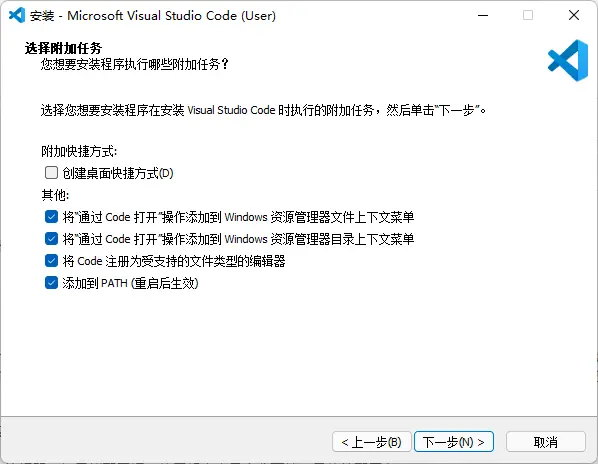
\includegraphics[width=8cm]{install-vs.png}
  \end{center}

\end{frame}

\begin{frame}{基础设置与 LaTeX Workshop 安装}
  \begin{enumerate}
    \item 更改语言为中文
    \item 安装 LaTeX Workshop
    \item 配置 LaTeX Workshop 编译链
    \item 更多内容:参见 \href{https://gitee.com/xkwxdyy/CCNUthesis/wikis/\%E5\%B8\%B8\%E8\%A7\%81\%E9\%97\%AE\%E9\%A2\%98FAQ/\%E5\%A6\%82\%E4\%BD\%95\%E5\%AE\%89\%E8\%A3\%85\%E3\%80\%81\%E9\%85\%8D\%E7\%BD\%AE\%E5\%92\%8C\%E4\%BD\%BF\%E7\%94\%A8VScode\#config-LW}{Wiki}. 
  \end{enumerate}
\end{frame}